\textbf{Problem 3}

The Ising model can be seen below, both the lattice and ``checkerboard'' are drawn. The checkerboard, as used as an example in the question, displays white tiles with label $w_i$ and black tiles with label $b_j$.

\begin{figure}[h]
	\centering
	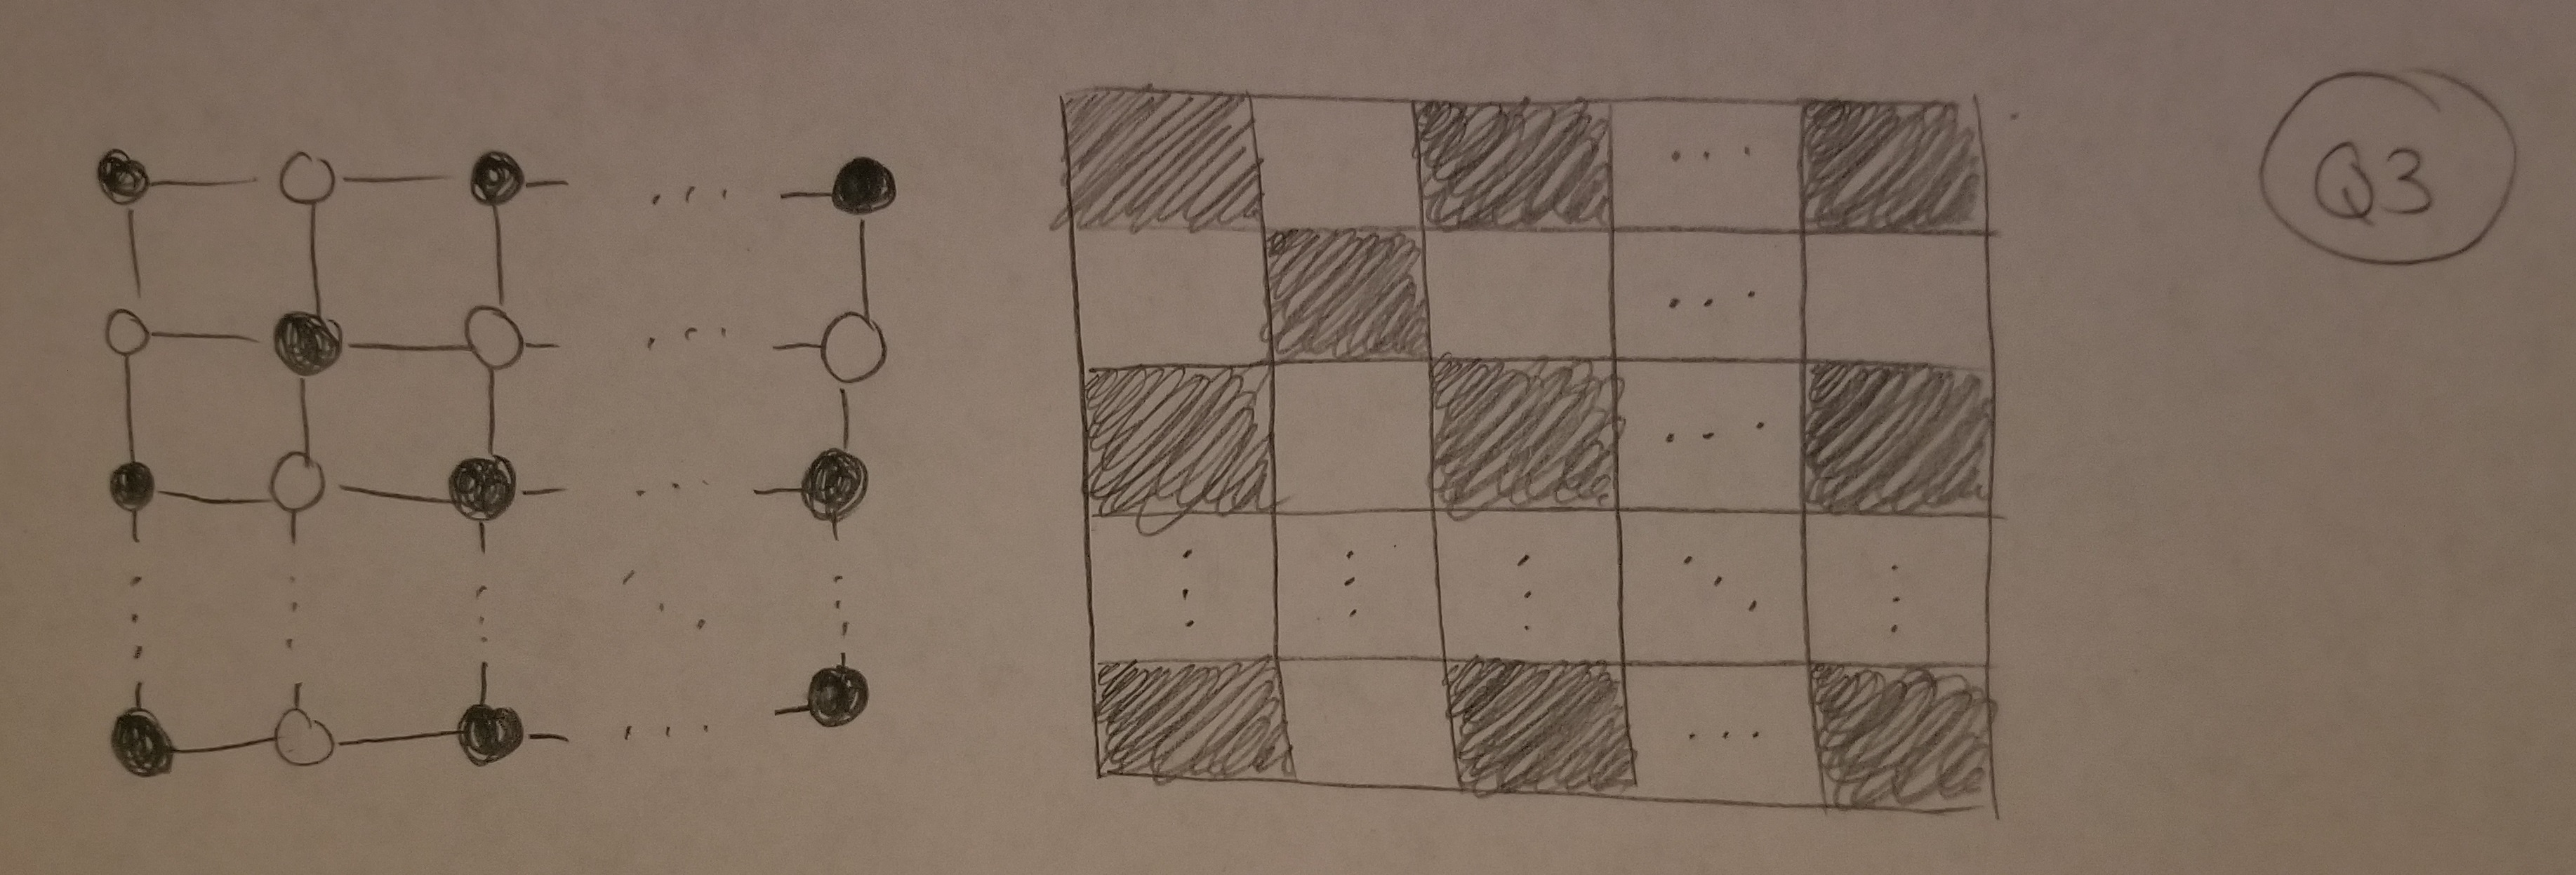
\includegraphics[scale=0.1]{q3-diagrams}
\end{figure}

We want to show that $p(b_1, b_2, \dots \vert w_1, w_2, \dots) = p(b_1 \vert w_1, w_2, \dots)p(b_2 \vert w_1, w_2, \dots)\dots$.

Assuming $p(x)$ represents the probability of a node $X$ being in state $x$ with neighbors $Y$, then because of nearest-neighbour interactions, we have $p(x \vert Y) = \exp(\beta \sum_{y_j \in Y} \mathbbm{1}[x_i = y_j])$. 

As such, this general idea can be carried over to the joint probability of the black tiles conditioned on the white tiles. Since each black tile only interacts with its neighbors (i.e. $Y = {w_1, w_2, \dots}$), which are white, we can easily see none of the black tiles are neighbours of each other. Since none of the black tiles are neighbors of each other, they cannot interact each other (i.e. black tiles do not interact with any other black tiles). Since there are no black-black interactions, we can assume they are independent. To put this in other words, when the white tiles are observed, they block any active trails between the black tiles, which makes the black tiles independent of one another. The opposite is also true (whites are independent of each other conditioned on blacks since there would be no active trails between whites). $\qed$

This above idea can be exploited by the Gibbs sampling procedure. In Gibbs sampling, we want to estimate some values $(x_1, x_2, \dots, x_n)$. For each iteration, we select some random variable $x_i$, and we want to make a guess/estimate for that variable's value, given the values of all the other variables, or in other words we want to estimate $x_i$ from the distribution $p(x_i \vert x_1, \dots, x_{i-1}, x_{i+1}, \dots, x_n) = p(x_i \vert x_{-i})$. Now, want to relate this ideology back to the original nearest-neighbour checkerboard example in this question. We are trying to estimate the distribution $p(b_1, b_2, \dots \vert w_1, w_2, \dots)$. Since we know the black tiles are independent of each other given the white variables, then assuming we are given values of the white variables, we can easily estimate each black tile's distribution $p(b_i \vert w_1, w_2, \dots)$ given the remaining black tile variables. Once we have sampled a given $b_i$, we can go back and sample $p(w_1, \dots, w_n \vert b_1, \dots, b_n)$ to get values for the white variables, and then go back in a loop and compute $p(b_1, \dots, b_n \vert w_1, \dots, w_n)$ again. So, clearly, since we can see the black variables are independent of each other given the white variables, we can fix the whites to sample the blacks, then fix the black variables to sample the white variables, and go back and forth in a loop to do Gibbs sampling.